\documentclass{article}

% Language setting
% Replace `english' with e.g. `spanish' to change the document language
\usepackage[english]{babel}

% Set page size and margins
% Replace `letterpaper' with `a4paper' for UK/EU standard size
\usepackage[letterpaper,top=2cm,bottom=2cm,left=3cm,right=3cm,marginparwidth=1.75cm]{geometry}

% Useful packages
\usepackage{amsmath}
\usepackage{amssymb}
\usepackage{graphicx}
\usepackage{booktabs}
\usepackage[colorlinks=true, allcolors=blue]{hyperref}
\usepackage{caption}
\usepackage{tabularx}
\usepackage{bm}
\usepackage{float}
\usepackage[font=small]{caption}
\usepackage{pythonhighlight}
\title{Your Paper}
\author{You}

\begin{document}
\maketitle

\newpage
\begin{abstract}

\end{abstract}

\section{Introduction}
Our situation is that we have obtained measurements, potentially noisy, of both
the $u$ and $f$. However, we do not have knowledge of the ODE parameters
$\phi$. This is a typical situation in for example lab work, where we have
measurements and want to determine an underlying physical parameter or
interpolate the data. This is often done with typical linear regression
techniques.\\ very easy to implement a better working kernel. one would always be able to build a better kernel for a specific problem. However this would require a lot of time and effort. with this framework we have a clear way of implementing a kernel that is based on the underlying physics. We do not need to analytically compute a kernel for a specific problem. We can just take the differential equation and a kernel and apply the differential operator to the kernel. This way we can easily implement a kernel for a specific problem. The next interesting thing is that we also use the knowledge of the forcing term for our prediction and for the calculation of the ODE hyperparameters $\phi$. and we can predict the forcing term aswell. When comparing this to a inverse problem using a neural network we can see that the implementation is also a lot harder.\\
We start with a general introduction to Gaussian Processes, Regression with Gaussian Processes and kernels. We
then introduce the physics informed framework and the optimization process. In the end we will look at several example problems and discuss the results and the performance of the framework.\\

\section{Fundamentals}
\subsection{Gaussian Process} %~\cite{pml1Book}\cite{RasmussenCarlEdward}
As defined in~\cite{RasmussenCarlEdward} a Gaussian Process is a collection of
random variables for which every finite set of variables have a joint
multivariate Gaussian distribution. For a Regression model we define a function
$f(\bm{x}): \mathcal{X}\rightarrow \mathbb{R}$ with the input set $\{\bm{X}\}$
= $\{\bm{x_n} \in \mathcal{X} \}_{n=1}^N$. We now let $f:
    \mathcal{X}\rightarrow \mathbb{R}$ be our Gaussian Process. To fully define the
GP we need to specify a mean function $m(\bm{x})$ and a covariance function or
kernel $k(\bm{x}, \bm{x'}): \mathcal{X} \times \mathcal{X} \rightarrow
    \mathbb{R}$ for $f(\bm{x})$:
\begin{equation}
    \begin{aligned}
        m(\bm{x})         & = \mathbb{E}[f(\bm{x})]                                    \\
        k(\bm{x},\bm{x'}) & = \mathbb{E}[(f(\bm{x})-m(\bm{x}))(f(\bm{x'})-m(\bm{x'}))]
    \end{aligned}
\end{equation}
In this work the mean function $m(\bm{x})$ of the GP is set to zero. This is quite common, mainly for notational reasons~\cite{RasmussenCarlEdward}.\\
So what we are left with for  $m(\bm{x})$ and $ k(\bm{x},\bm{x'})$ is:
\begin{equation}
    \begin{aligned}
        m(\bm{x})         & = 0                               \\
        k(\bm{x},\bm{x'}) & = \mathbb{E}[f(\bm{x})f(\bm{x'})]
    \end{aligned}
\end{equation}
We now write our Gaussian Process $f(\bm{x})$ as:
\begin{equation}
    f(\bm{x})\thicksim \mathcal{G} \mathcal{P}(0,k(\bm{x},\bm{x'}))
\end{equation}
It is important to note that $ k(\bm{x},\bm{x'})$ has to be positive definite and symmetric in order to be a valid kernel function.
Because of the definition of the GP we can now generate a joint Gaussian distribution for a finite set of points $\bm{X_*}$:
\begin{equation}
    \label{eq:f_star_random_vector}
    p(\bm{f_*|\bm{X_*}}) = \mathcal{N}(\bm{f_*}|\bm{0},\bm{K_*})
\end{equation}
with ${[\bm{K}]}_{i,j} = k(\bm{x_{i*}},\bm{x_{j*}})$.

\subsection{Regression}\label{sec:Regression}
The goal of regression is given a training dataset $\mathcal{D} =
    \{(\bm{x_i},y_i)|i = 1,\ldots,N\}$ we want to make predictions for new test
points $\bm{x_*}$ which are not in the training set. There are several methods
which can be used to tackle this kind of problem. For example the basic linear
regression using least squares and specific basis functions or a neural network
that does regression. In this work we make use of the Gaussian process which is
a non-parametric model. We will start with a Gaussian Process prior and then
use the rules for Gaussian multivariate distributions to define a posterior
predictive distribution, which we can then use to make predictions for new test
points.

The general setup for regression is that we make observations/measurements $y$
of an underlying function $f(\bm{x})$ at points $\bm{x}$ which are corrupted by
a zero mean Gaussian noise with variance $\sigma_n^2$:
\begin{equation}
    \bm{y} = \bm{f}(\bm{X}) + \mathcal{N}(0|\sigma_n^2 \bm{I})
\end{equation}
When we set the GP Prior onto the function $f$ we have to add the normally distributed noise. To get the prior for the observations $\bm{y}$ we simply need to change the covariance function to cov($\bm{y_p,y_q}$) = $k(\bm{x_p,x_q}) + \sigma_n^2\delta_{pq}$.\\
As described before in equation~\ref{eq:f_star_random_vector} we can generate a Gaussian random vector for new test data $\bm{X_*}$. Both $\bm{y}$ and $\bm{f_*}$ are now multivariate Gaussians. We can therefore introduce the joint distribution of the observed data and the values of $f$ at the test points $\bm{X_*}$ as:
\begin{equation}
    \label{eq:joint_f,X_*}
    \begin{aligned}
        \begin{bmatrix}
            \bm{y} \\
            \bm{f_*}
        \end{bmatrix}
        \thicksim  \mathcal{N}\left(\bm{0},
        \begin{bmatrix}
            K(\bm{X},\bm{X}) + \sigma_n^2 \bm{I} & K(\bm{X},\bm{X_*})   \\
            K(\bm{X_*},\bm{X})                   & K(\bm{X_*},\bm{X_*})
        \end{bmatrix}
        \right)
    \end{aligned}
\end{equation}
From this joint Gaussian prior we can then calculate the predictive posterior distribution by applying the rules for conditioning Gaussians. A good description for this conditioning can be found in~\cite{bishop} (chapter 2.3.1). The predictive distribution is then given by:
\begin{equation}
    \begin{aligned}
        \label{eq:general_kernel}
        p(\bm{f_*}|\bm{X},\bm{y},\bm{X_*}) & = \mathcal{N}(\bm{f_*|\bm{\mu_*}},\bm{\Sigma_*})                                                           \\
        \bm{\mu_*}                         & =  K(\bm{X_*},\bm{X}){[K(\bm{X},\bm{X}) + \sigma_n^2 \bm{I}]}^{-1} \bm{y}                                  \\
        \bm{\Sigma_*}                      & = K(\bm{X_*},\bm{X_*}) - K(\bm{X_*},\bm{X}){[K(\bm{X},\bm{X}) + \sigma_n^2 \bm{I}]}^{-1}K(\bm{X},\bm{X_*})
    \end{aligned}
\end{equation}
We now have obtained the posterior predictive mean $\bm{\mu_*}$ and the posterior covariance $\sigma$ for the new test inputs $\bm{X_*}$.

\subsection{Kernels}
In~\cite{RasmussenCarlEdward} a kernel is defined as a function
$k(\bm{x},\bm{x'})$, which maps two input pairs $\bm{x} \in \mathcal{X}$ and
$\bm{x'} \in \mathcal{X'}$ into $\mathbb{R}$. To be a valid covariance function
the kernel needs to satisfy two main conditions. First it needs to be symmetric
so that $k(\bm{x,x'}) = k(\bm{x,x'})$ and second it needs to be positive
semidefinite (PSD) The general covariance function used in this work is the
squared exponential covariance function (SE) as defined
in~\cite{RasmussenCarlEdward}:
\begin{equation}
    k(\bm{x_p}, \bm{x_q}) = \sigma_f^2  \exp({-0.5{(\bm{x_p}-\bm{x_q} )}^\intercal M (\bm{x_p}- \bm{x_q})})
\end{equation}
with the variance hyperparameter $\sigma_f^2$ and the matrix $M = {\mathrm{diag}(\bm{l})}^{-2}$ containing the vector with the characteristic length scales $l_i$. The hyperparameters are collected in the vector $\bm{\theta} = (\bm{l},\sigma_f^2)$. \\
For the one dimensional case the SE covariance function simply becomes:
\begin{equation}
    k(x_p, x_q) = \sigma_f^2  \exp\left({-\frac{0.5}{l^2} {(x_p-x_q)}^2}\right)
\end{equation}
For a two-dimensional case with time being the second dimension, two independent length scale parameters are used for the separate space and time domains $\bm{l} = (l_x,l_t)$. For this case, we can re-write equation~\ref{eq:general_kernel} the covariance function with $\bm{x_p} = {(x_p, t_p)}^\intercal$ and  $\bm{x_q} = {(x_q, t_q)}^\intercal$ as the product of two single SE covariance functions:
\begin{equation}
    k(\bm{x_p}, \bm{x_q}) = \sigma_f^2  \exp\left({-\frac{0.5}{l_x^2} {(x_p-x_q)}^2}\right) \exp\left({-\frac{0.5}{l_t^2} {(t_p-t_q)}^2}\right)
\end{equation}
There are many kernels one can choose from. A good overview over some kernel functions, as well as how they can be modified, can be found in~\cite{Duvenaud} as well as in~\cite{görtler2019a}. Later we will modify the SE kernels with linear operators, more specifically with differential operators. For this the SE kernel is a good choice, because it is infinitely differentiable with rather simple and smooth derivatives. This is important for the overall numerical stabililty when calculating the gradients of the modified kernel in the optimization process.\\ 
\subsection{Marginal likelihood}

For the optimization of the hyperparameters $\theta$ and $\phi$ the negative
marginal log likelihood ($nmll$)~\cite{RasmussenCarlEdward} is minimized. The
$nmll$
\begin{equation}
    \log p(\bm{y}|\bm{X},\bm{\theta}) = -\frac{1}{2}\bm{y}^\intercal \bm{K_y}^{-1}\bm{y} - \frac{1}{2}\log\left\lvert \bm{K_y}\right\rvert - \frac{n}{2}\log(2\pi)
\end{equation}
with $K_y$ = $K_f + \sigma_n^2 \bm{I}$. As described in~\cite{RasmussenCarlEdward}, the $mll$ consists of three parts, which can each be understood separately. The first term $\frac{1}{2}\bm{y}^\intercal \bm{K_y}^{-1}\bm{y}$ is in charge of the data fit, the second term $\log\left\lvert K_y\right\rvert$ is the complexity penalty and the last term is a normalization term.

\subsection{Linear operators and GPs}
A useful property of Gaussian Processes is that their linear transformation is
still a Gaussian Process. This main

\section{Physics informed framework}
We choose our problem setup similar/eual to the one proposed in~\cite{RAISSI}. At the top we 
have some sort of linear differential equation of a physical model:
\begin{equation}
    \label{eq:Lu=f}
    \mathcal{L}_{\bm{x}}^\phi u(\bm{x}) = f(\bm{x})
\end{equation}
which can be written as a linear operator $\mathcal{L}_{\bm{x}}^\phi$ acting on the function $u(\bm{x})$. $\mathcal{L}_{\bm{x}}^\phi$ is a differential operator that resembles the differential equation with $\phi$ being a list containing the a-priori unknown parameters which also define the differential equation. The function $f(\bm{x})$ acts as the forcing term and $u(\bm{x})$ is the solution of the differential equation.  \\
\\
We now start by assuming that the solution of the differential equation $u(\bm{x})$ is a Gaussian Process of the form:
\begin{equation}
    u(\bm{x}) \thicksim \mathcal{G}\mathcal{P}(\bm{0},k_{uu}(\bm{x},\bm{x'};\bm{\theta}))
\end{equation}
with $k_{uu}(\bm{x},\bm{x'};\bm{\theta})$ being the kernel depending on its hyperparameters $\theta$ for the $\mathcal{G}\mathcal{P}$ (on) $u(\bm{x})$. With the known linear relation between $u$ and $f$ from equation~\ref{eq:Lu=f}, we can now say that $f(\bm{x})$ must also be $\mathcal{G}\mathcal{P}$~\cite{RasmussenCarlEdward} of form:
\begin{equation}
    f(\bm{x}) \thicksim \mathcal{G}\mathcal{P}(\bm{0},k_{ff}(\bm{x},\bm{x'};\bm{\theta}))
\end{equation}
with now $k_{ff}$ being the kernel defining the $\mathcal{G}\mathcal{P}$ (on) $f(\bm{x})$. As shown in~\cite{garnett_2023_full},~\cite{Särkkä} and~\cite{RAISSI} $k_{ff}$ is defined by:
\begin{equation}
    k_{ff}(\bm{x},\bm{x'};\bm{\theta}, \bm{\phi}) = \mathcal{L}_{\bm{x}}^\phi \mathcal{L}_{\bm{x'}}^\phi k_{uu}(\bm{x},\bm{x'};\bm{\theta})
\end{equation}
We also need the mixed terms between $u(x)$ and $f(x)$, namely $k_{uf}$ and $k_{fu}$ which are formed by:
\begin{equation}
    \begin{aligned}
        k_{uf}(\bm{x,x'};\bm{\theta,\phi}) & = \mathcal{L}_{\bm{x'}}^\phi k_{uu}(\bm{x},\bm{x'};\bm{\theta}) \\
        k_{fu}(\bm{x,x'};\bm{\theta,\phi}) & = \mathcal{L}_{\bm{x}}^\phi k_{uu}(\bm{x},\bm{x'};\bm{\theta})
    \end{aligned}
\end{equation}
To simplify the notation, the dependence on the hyperparameters $\bm{\theta}$ and $\bm{\phi}$ is not written explicitly anymore.
With this construction we now have two Gaussian Processes. As described in~\cite{garnett_2023_full} we can now create a joint Gaussian process of u and f in the form: (not sure if I understood this correctly)
\begin{equation}
    \label{eq:jointGP}
    \begin{aligned}
        \begin{bmatrix}
            u \\
            f
        \end{bmatrix}
    \end{aligned}
    \thicksim \mathcal{GP}\left(\bm{0},
    \begin{bmatrix}
        k_{uu} & k_{uf} \\
        k_{fu} & k_{ff}
    \end{bmatrix}\right)
\end{equation}
with $k_{uu}: \mathcal{U} \times  \mathcal{U}$, $k_{uf}: \mathcal{U} \times  \mathcal{F}$, $k_{fu}: \mathcal{F} \times  \mathcal{U}$ and $k_{ff}: \mathcal{F} \times  \mathcal{F}$
We now look at noisy observations of both $u$ and $f$,with noise $\sigma_u$ and $\sigma_f$, of the form:
\begin{equation}
    \begin{aligned}
        y_{i,u} = u_i(\bm{x_{i,u}}) + \mathcal{N}(0|\sigma_u^2) \\
        y_{i,f} = u_i(\bm{x_{i,f}}) + \mathcal{N}(0|\sigma_f^2)
    \end{aligned}
\end{equation}
with which we create two data sets $\{\bm{X_u,y_u}\}$ and $\{\bm{X_f,y_f}\}$. Similarly, as we did before for the test points in equation~\ref{eq:joint_f,X_*} we can now write (create) a joint Gaussian distribution of the observations $\bm{y_u}$ and $\bm{y_f}$. We collect $\bm{X_u,X_f}$ in $\bm{X}$ and $\bm{y_u,y_f}$ in $\bm{y}$. With the joint GP at equation~\ref{eq:jointGP}, the joint distribution will take the following form:
\begin{equation}
    \label{eq:jointGP_observations}
    \begin{aligned}
        p(\bm{y}|\bm{X},\bm{\theta},\sigma_{n_u}^2,\sigma_{f_u}^2,\bm{\phi}) =
        \mathcal{N}\left(\bm{0},
        \begin{bmatrix}
            k_{uu}(\bm{X_u,X_u}) + \sigma_{n_u}^2 \bm{I} & k_{uf}(\bm{X_u,X_f})                         \\
            k_{fu}(\bm{X_f,X_u})                         & k_{ff}(\bm{X_f,X_f}) + \sigma_{n_f}^2 \bm{I}
        \end{bmatrix}\right)
    \end{aligned}
\end{equation}

We can directly use $\bm{K}$ to compute the mag log likelihood and train the
model to obtain the optimized hyperparameters $\bm{\theta_*}$ and
$\bm{\phi_*}$. More information about the optimization process will be provided
in the next chapter.

\subsection{Optimization/Finding of the hyperparameters}
Arguably the most important part of the overall framework is the optimization of the hyperparameters. The optimization is done by minimizing the negative marginal log likelihood (mll) of the joint GP with respect to the hyperparameters $\bm{\theta, \phi}$. The mll is defined as:
\begin{equation}
    \log p(\bm{y}|\bm{X},\bm{\theta},\sigma_{n_u}^2,\sigma_{f_u}^2,\bm{\phi}) =
    -\frac{1}{2}\bm{y}^\intercal \bm{K}^{-1}\bm{y} - \frac{1}{2}\log\left\lvert \bm{K}\right\rvert - \frac{n}{2}\log(2\pi)
\end{equation}
with $\bm{K}$ being the covariance matrix of the joint GP in equation~\ref{eq:jointGP_observations}. For the optimization we tried different gradient based optimizers, aswell as a heuristic search method, namely the Nelder-Mead method. All the optimizers used came from the scipy.optimize.minimize function from the scipy library. We tried several gradient based optimizers like the limited memmory Broyden-Fletcher-Goldfarb-Shanno (L-BFGS-B) algorithm, the conjugate gradient (CG) algorithm and the truncated Newton (TNC) algorithm. The best results were however obtained by using the Nelder-Mead~\cite{Singer:2009NelderMead}. From the gradient based methods the TNC performed the best and was most of the time nearly as good as the Nelder-Mead. However, the TNC was significantly slower and needed more restarts than the Nelder-Mead. Especially with an increasing number of training points the gradient based optimizers failed completly and the Nelder-Mead method was the only one that still worked. This could be because the Nelder Mead algorithm does not use any gradient information and that for more training points the calculation of the gradients of the mll gets unstable. Generally, it is important to add some jitter to the diagonal of $\bm{K}$ to minimize the risk of numerical instabilities when calcualting the Cholesky decomposition of $\bm{K}$. Also, without jitter a significant part of the optimization landscape is not defined, because of the  gram matrix $\bm{K}$ not beeing positive definite for some hyperparameter values. The best results were obtained when using a jitter in the range of $10^{-6} to 10^{-7}$\\
\\
A common problem in the optimization process of non-convex funtion is the problem of converging to a local minimum. To avoid this problem we started the optimization process for different initial values of the hperparameters. The initial values were sampled from uniform distributions, only the length scale hyperparameter $l$ was sampled from a log uniform distribution because of it beeing a scale parameter. Because of the random initialization, and the presumably high number of local minima in the optimization landscape, the results for the hyperparameters varied. However, for a sufficient number of optimization runs the results normally reached a similar accuracy and similar hyperparamter values.\\
\\
To conclude, the optimization process is the key part of the framework, because we can directly make predictions with the optimized hyperparameters, but also obtain the parameters $\phi$ of the underlying differential equation. A key step for improving the overall framework would be to improve the optimization process. However, this would be very time consuming and the obtained results are sufficently accurate, aswell as the computation time beeing reasonably short, for the scope of this work.\\
\subsection{Predictions with the Posterior}
With the obtained hyperparameters $\bm{\theta_*}$ and $\bm{\phi_*}$ we can make
new predictions at a test location $\bm{x_*}$. Similar to the construction in
chapter~\ref{sec:Regression} we can now formulate the predictive posterior
distribution for $u(\bm{x_*})$ and also for $f(\bm{x_*})$ as done
in~\cite{RAISSI}:
\begin{equation}
    \begin{aligned}
        p(u(\bm{x_*})|\bm{y},\bm{X},\bm{\theta_*}, \bm{\phi_*}) = \mathcal{N}(\mu_{u*}, \Sigma_u) \\
        p(u(\bm{x_*})|\bm{y},\bm{X},\bm{\theta_*}, \bm{\phi_*}) = \mathcal{N}(\mu_{f*}, \Sigma_f)
    \end{aligned}
\end{equation}
with
\begin{equation}
    \begin{aligned}
        \label{eq:predictive_mean_cov}
        \mu_u = \bm{\kappa_u}\bm{K}^{-1}\bm{y}, \; \Sigma_* = k_{uu}(\bm{x_*,x_*}) - \bm{\kappa_u}\bm{K}^{-1}\bm{\kappa_u}^\intercal  \\
        \mu_f = \bm{\kappa_f}\bm{K}^{-1}\bm{y}, \;  \Sigma_* = k_{ff}(\bm{x_*,x_*}) - \bm{\kappa_f}\bm{K}^{-1}\bm{\kappa_f}^\intercal \\
    \end{aligned}
\end{equation}
with $\bm{\kappa_u}$ and $\bm{\kappa_f}$ being:
\begin{equation}
    \begin{aligned}
        \bm{\kappa_u} = [k_{uu}(\bm{x_*},\bm{X_u})k_{uf}(\bm{x_*,\bm{X_f}})] \\
        \bm{\kappa_f} = [k_{fu}(\bm{x_*},\bm{X_u})k_{ff}(\bm{x_*,\bm{X_f}})]
    \end{aligned}
\end{equation}
For the actual implementation we again used the Cholesky decomposition of $\bm{K}$ to compute the inverse of $\bm{K}$. This is done by first computing the Cholesky decomposition of $\bm{K}$:
\begin{equation}
    \bm{K} = \bm{L}\bm{L}^\intercal
\end{equation}
with $\bm{L}$ being a lower triangular matrix. We can then write equation \ref{eq:predictive_mean_cov} as:
\begin{equation}
    \begin{aligned}
        \mu_i = \bm{\kappa_i} \bm{L^{\intercal} \backslash (L\backslash y)}, \; \Sigma_i = k_{ii}(\bm{x_*,x_*}) - \bm{\kappa_i} \bm{L^{\intercal} \backslash (L\backslash \kappa_i^{\intercal})}
    \end{aligned}
\end{equation}
with $\backslash$ as the left matrix divide operator. This is a stable way of computing the inverse of $\bm{K}$. This way of calculating the predictive mean and covariance is also used in \cite{RasmussenCarlEdward} and \cite{RAISSI}.

\section{Results}
In the following we will call the physics informed model, which is used here the
informed model and the vanilla model the model without the physics informed
framework and only a general SE kernel.\\ \\ For testing the framework we will
use ODEs and PDEs of physical models. More specifically, we will look at the
three main types of PDEs, namely the Elliptic, Hyperbolic, and Parabolic type and as a starting example a damped oscillator in one dimension. For obtaining
$u(\bm{x})$, we will fully define the differential equation with its initial-
and boundary conditions and then use mathematicas NDSolve (numerical solution)
or NSolve (analytical solution) to compute the solution
$\{(\bm{x});u(\bm{x}),f(\bm{x})\}$. The obtained solutions will be used as the ground truth.
The training and validation points will be sampled from the solution domain $[\bm{x}_{\min}, \bm{x}_{\max}]$ using a sobol
sequence[cite]. We will add some noise to the samples for the training and
validation points, to analyse the impact onto the results and to simulate real
world data. Furthermore, often the incoporation of a small noise improves stability in
the optimization and prediction process. This will be done by creating two data
sets $\{(\bm{x_u});\bm{y_u}\}$ and $\{(\bm{x_f});\bm{y_f}\}$ with $\bm{y_i} =
    u(\bm{x_i}) + \mathcal{N}(\bm{0}|\sigma_{ni}^2 I) ; \; i = u,f$. The
implementation of a sobol sequence helps with evenly spaced training and
validation points, which is important for the training process of the model.\\
Through the optimization of the mll, we will obtain the parameters of the
underlying equation $\phi$, as well as the hyperparameters $\theta$ of the
kernel. With these parameters we will then calculate the predictive mean and
covariance and then compare the ground truth with the computed mean function.
To quantify/benchmark the performance we will look at the marginal log likelihood, the mean squared error (MSE) and the relative L2 error of the validation set(ground truth). As another
way of looking at the performance of the informed model we will compare it to a
vanilla model with a general SE kernel, as described in~\ref{sec:Regression}.
For this we will use the GPy library~\cite{gpy2014}. However, it is important
to acknowledge that the vanilla model with the simple SE kernel only has two/three (for cases with time as a second dimension) hyperparameters, namely the length scale $l$ and the variance $\sigma_f^2$.
Additionaly, the informed model takes advantage of the joint GP. This means
that the informed model has more parameters to optimize and additional
information from the joint GP, and therefore it is not a fair comparison.
However, it is still interesting to see how the informed model performs
compared to the vanilla model and to have a general benchmark. To further
investiage this we will give one exmaple with the same amount of
hyperparameters, namely the Poisson equation and compare the results of the two
models.\\
\subsection{Damped oscillator}
As a first example we will look at a one dimensional differential equation of a
damped oscillator with mass $m$, damping $\gamma$ and force constant $k$. The
differential equation is given by:
\begin{equation}
    \begin{aligned}
        m\frac{\partial^2 u(t)}{\partial t^2} + \gamma \frac{\partial u(t)}{\partial t} + k u(t) = f(t) \\ u(0) = 0, \; \frac{\partial u(t)}{\partial t} = 0
    \end{aligned}
\end{equation}
The first data set was generated with $m = 1, \gamma = 2, k = 2$ and a simple sinusoidal forcing term $f(t) = 4 \sin(2\pi t)$. For the added noise we used $\sigma_{nu} = 10^{-4}$ and $\sigma_{nf} = 10^{-4}$ which can be seen as noise free data. We calculated the result in the time interval $t \in [0,3]$ from with we sample the training points. The model learns the hyperparameters $\bm{\theta}$ $(l,\sigma_f,m,\gamma,k)$ to be $(0.4890, 0.5860, 0.9989, 1.9925, 1.9987)$. These results are very accurate considering we are only using 9 training points for a model with 5 hyperparameters. As elaborated before, the exact value of the final values after optimizing varies in a small range. The predictive distribution for the general solution $u(t)$ and the forcing term $f(t)$ can be seen in figure~\ref{fig:damped_oscillator}. Looking at the results for the informed model we can see that the prediction for $u(t)$ and for $f(t)$ are very precise. The posterior mean overlines with the validation points and the uncertanty band is so small that is not even visible. The mean squared error of $u(t)$ and $f(t)$ are $MSE_u = 1.419 \cdot 10^{-7}$ and $MSE_f = 4.609 \cdot 10^{-3}$. The predictive mean of the vanilla model can also be seen in figure~\ref{fig:damped_oscillator}. The MSEs for the vanilla model are $MSE_{u,va} = 5.469 \cdot 10^{-4}$ and $MSE_{f,va} = 2.692$. The MSE for the vanilla model is 3 to 4 orders of magnitude higher than the MSE of the informed model which gets very clear when looking at figure~\ref{fig:damped_oscillator}. The predictions from the vanilla model are not very precise with large uncertanties. This is also reflected in the MSEs. The informed model even manages to accuratly predict in areas away from any training points, as well as at the edges of the domain.
\begin{figure}[htbp!]
    \centering
    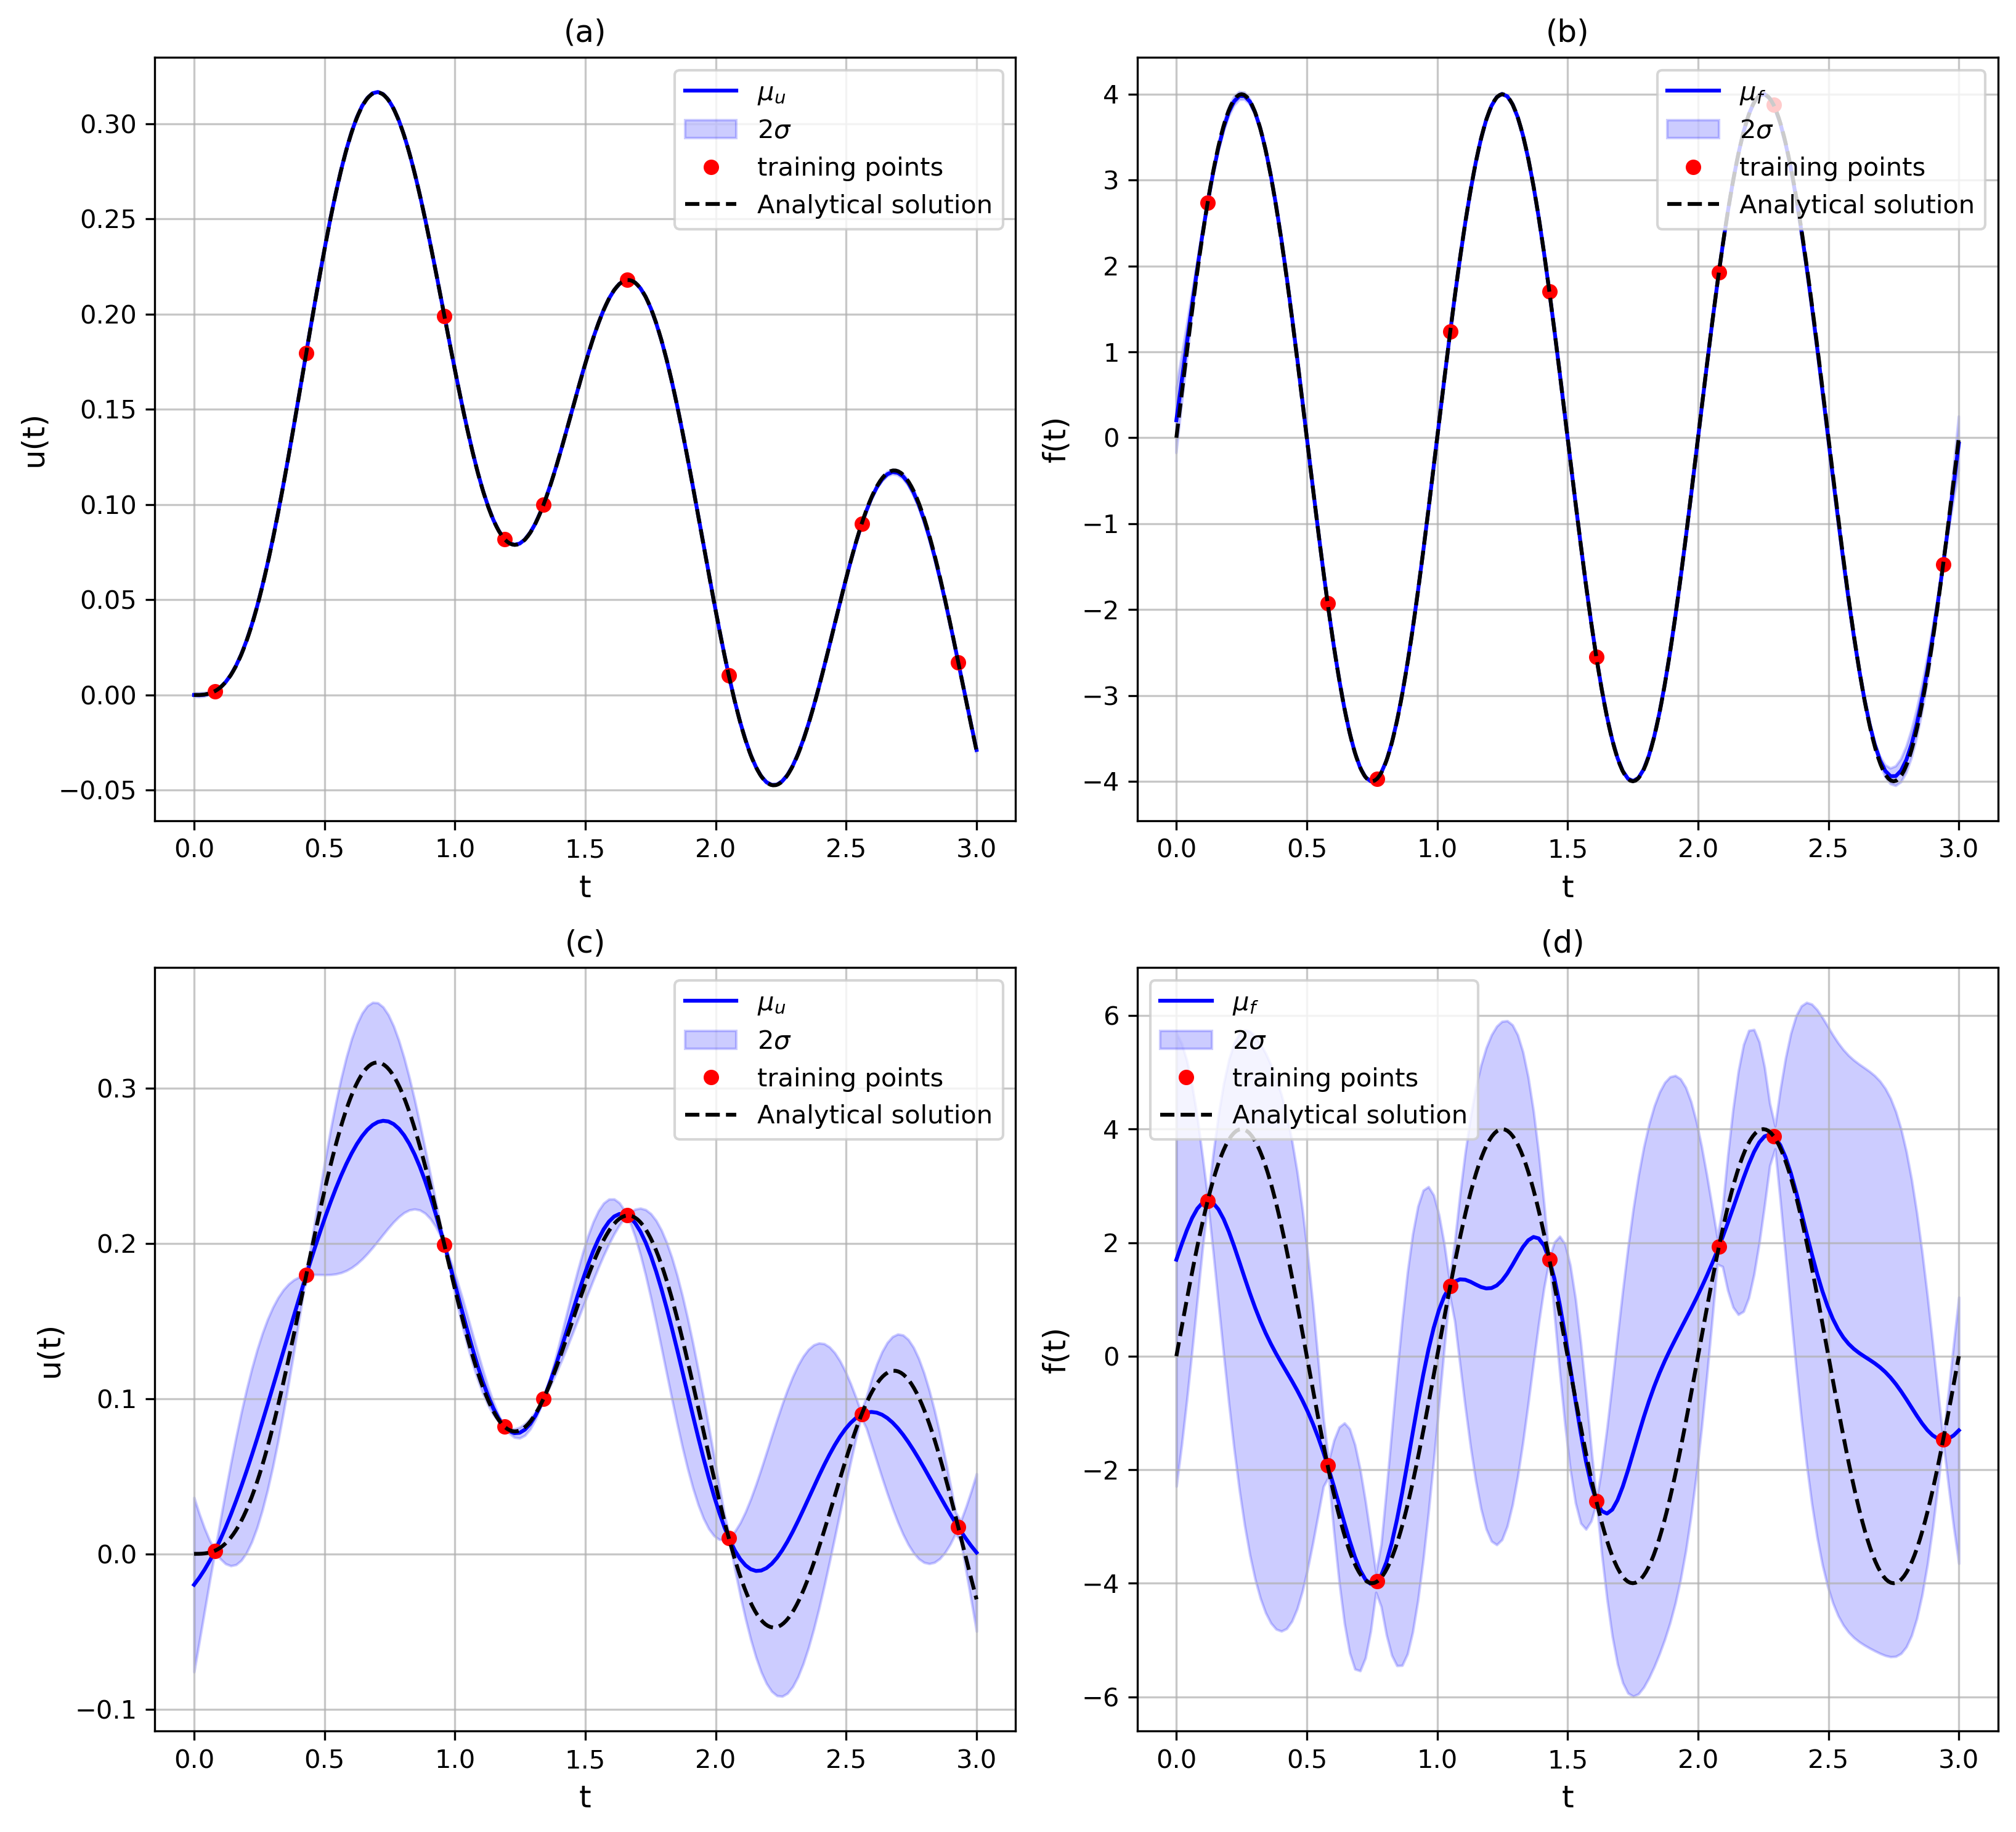
\includegraphics[width=1\textwidth]{../final_examples/oscillator/merged_1d_plots.png}
    \caption{(a) \& (b) predictive mean $\mu_u$ and $\mu_f$ for the informed model, two $\sigma$ uncertanty band, training and validation points sampled from $\{\bm{x_u},u(\bm{y_u})\}$ and $\{\bm{x_f},u(\bm{y_f})\}$ respectivly.\ (c) \& (d) predictive mean $\mu_u$ and $\mu_f$ for the vanilla model, two $\sigma$ uncertanty band, training and validation points sampled from $\{\bm{x_u},u(\bm{y_u})\}$ and $\{\bm{x_f},u(\bm{y_f})\}$ respectivly. The noise $\sigma_{nu}$ and $\sigma_{nf}$ were both set to $10^{-8}$. The MSEs of the informed model are $MSE_u = 1.419 \cdot 10^{-7}$ and $MSE_f = 4.609 \cdot 10^{-3}$. The MSEs for the vanilla model are $MSE_{u,va} = 5.469 \cdot 10^{-4}$ and $MSE_{f,va} = 2.692$.}
    ~\label{fig:damped_oscillator}
\end{figure}
\\
To investiagete the impact of noise we will look at the same example as before, but with added noise. We will use $\sigma_{nu} = $ and $\sigma_{nf}$. This is a significant amount of noise, but the model still manages to predict the hyperparameters as $(,,)$
To benchmark the performance further we looked at cases with different numer of training points. The results can be seen in table~\ref{tab:variing_n_trainingpoints}.
\begin{table}[htbp!]
    \caption{MSEs for the informed model with different number of training points $n$. The used noise was $\sigma_{nu} = $ and $\sigma_{nf}$.}
    \centering
    \begin{tabular}{ccccc}
        \toprule
        $n$     & 5 & 10 & 20 & 50 \\
        \midrule
        $mll$ &   3.722&  -10.049  &   -53.227 &  -32.808 \\
        $L²_u$& & & & \\
        $L²_f$ & & & & \\
        $MSE_u$ & 5.583 $\cdot 10^{-3}$  &  1.070 $\cdot 10^{-7}$  &  2.463 $\cdot 10^{-8}$  &   4.022 $\cdot 10^{-8}$ \\
        $MSE_f$ &  4.974 & 2.347 $\cdot 10^{-3}$  & 1.076 $\cdot 10^{-3}$ &  0.105 \\
        \bottomrule
    \end{tabular}
    
    \label{tab:variing_n_trainingpoints}
\end{table}
\subsection{Heat Equation}
The one dimensional time dependent heat equation with a forcing term is:
\begin{equation}
    \begin{aligned}
        \frac{\partial u(x,t)}{\partial t} - \alpha \frac{\partial^2 u(x,t)}{\partial x^2} = f(x,t) \\ u[0,x] =\\ u(t,0) = ; u(t,L) =
    \end{aligned}
\end{equation}
with $\alpha$ as the thermal diffusivity.


\subsection{Wave Equation}
For the second example we will look at the one dimensional time dependent wave equation. The wave equation is a hyperbolic partial differential equation that describes the propagation of waves of various types. In our case we can think of the wave equation as a string that is fixed at both ends. The wave equation is given by:
\begin{equation}
    \begin{aligned}
        \frac{1}{c^2} \frac{\partial^2 u(x,t)}{\partial t^2} - \frac{\partial^2 u(x,t)}{\partial x^2} = f(x,t) \\ u[0,x] =\\ u(t,0) = ; u(t,L) =
    \end{aligned}
\end{equation}
with $c$ as the wave speed. The ground truth was calculated with $c = 3$ and with $f(x,t) = $. We used 20 training points for both $u$ and $f$. The training data was sampled from the domain $x \in [0,1]$ and $t \in [0,1]$. The noise was set to $\sigma_{nu} = 10^{-4}$ and $\sigma_{nf} = 10^{-4}$, which can be considered as nearly noise free. The hyperparameters ($l_x$, $l_t$,$\sigma_f$, $c$) were optimized to be $(,,)$.
\begin{figure}
    \centering
    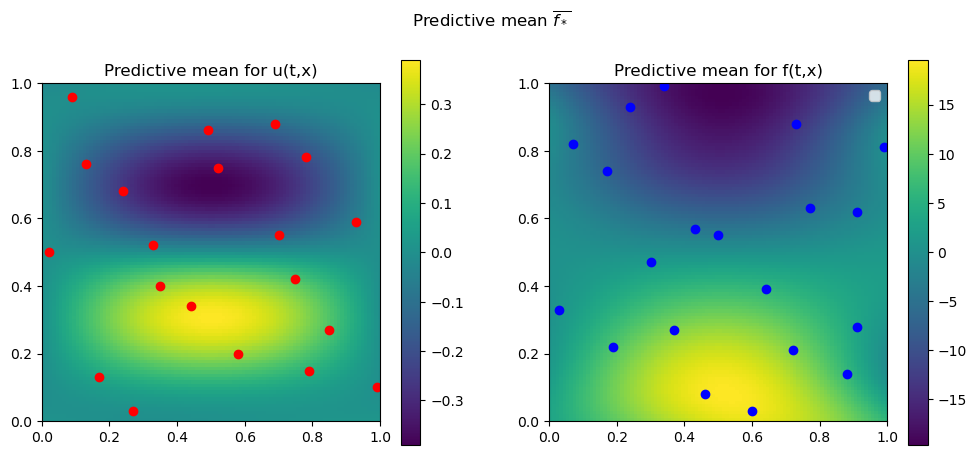
\includegraphics[width=1\textwidth]{../final_examples/wave_equation/predictive_mean.png}
    \caption{Plots for the informed model. (a) \& (b) predictive mean $\bm{\mu_u}$ and $\bm{\mu_f}$ with training points in red. (c) \& (d) predictive standard deviations $\bm{\sigma_u}$ and $\bm{\sigma_f}$. (e) \& (f) difference between the predictive mean $\bm{\mu}$ and the ground truths $u$ and $f$. The MSEs for the informed model are $MSE_u =  \cdot 10^{-7}$ and $MSE_f =  \cdot 10^{-3}$. The relative $L²$ errors are $L^2_u = $ and $L^2_f = $.}
    ~\label{fig:wave}
\end{figure}
\subsection{Poisson Equation}
In our last example we will look at a case where we do not incorporate additional ODE parameters $\phi$ in the form of hyperparameters into the kernel. This is to better look at the general predictive performance of the informed model in comparison to the vanilla model. The informed, aswell as the vanilla model will both not incorporate ARD, therefore there will only be one singel length scale $l$ for both spatial dimensions. With this example we now have the same amount of optimizable hyperparameters. \\
\\
 We will look at the Poisson equation in two spatial dimensions with a
forcing term and with dirichlet boundary conditions:
\begin{equation}
    \begin{aligned}
        \nabla^2 u(x,y) = f(x,y) \\ u[0,x] = \\ u(t,0) = 0; u(t,L) = 0
    \end{aligned}
\end{equation}


 Overall, the performance of the infomed model is significantly better. The relative error for $L²_u$ is and $L²_f$ is. The predictive mean, the predictive variance and the calculated difference between the prediction and the ground truth are shown in figure \ref{fig:poisson}. Comparing this to the vanilla model with relative errors of $L²_u = 0.0989$ and $L²_f = 0.0728$ we can see that the informed model is more than an order of magnitude more accurate. The predictive mean and the difference to the ground truth can be seen in figure \ref{fig:poisson_GPY}. The better prediction is also reflected in the MSEs. The MSEs for the informed model are $MSE_u = . \cdot 10^{-7}$ and $MSE_f =  \cdot 10^{-3}$. The MSEs for the vanilla model are $MSE_{u,va} = 9.862  \cdot 10^{-5}$ and $MSE_{f,va} = 0.130$.\\
\\
\begin{figure}[htbp!]
    \centering
    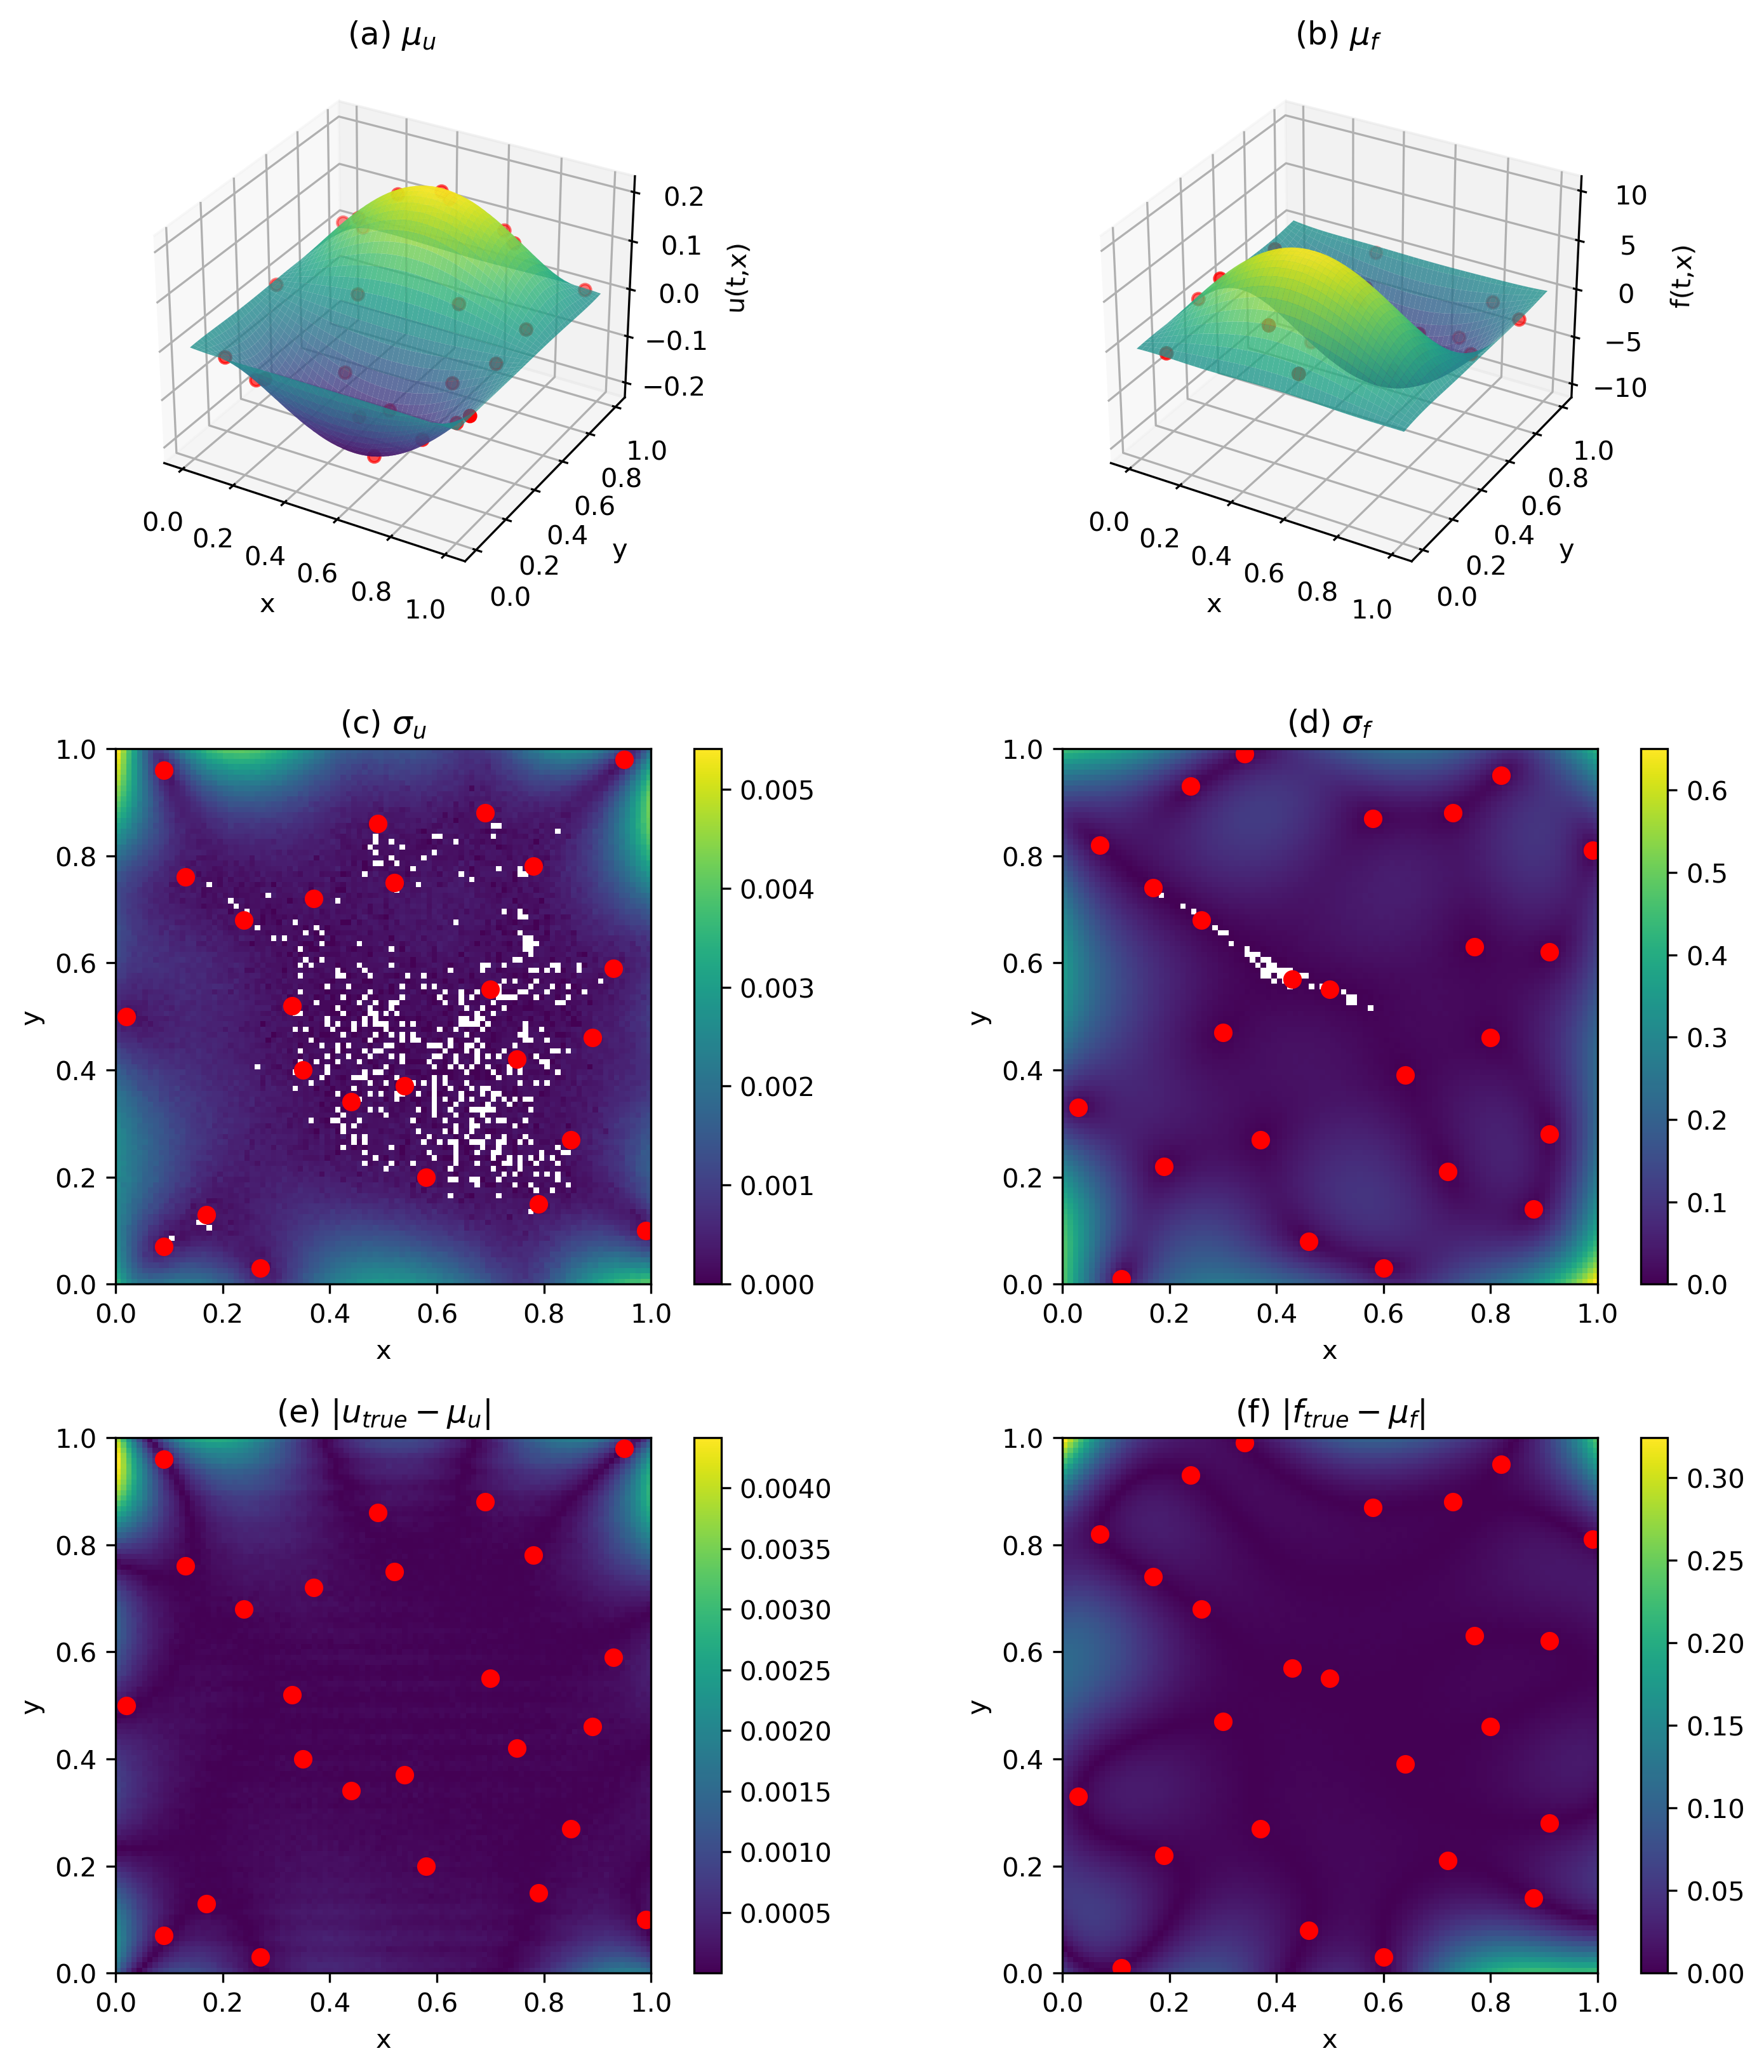
\includegraphics[width=1\textwidth]{../final_examples/poisson/merged_2d_plots.png}
    \caption{Plots for the informed model. (a) \& (b)  predictive mean $\bm{\mu_u}$ and $\bm{\mu_f}$ with training points in red. (c) \& (d) predictive standard deviations $\bm{\sigma_u}$ and $\bm{\sigma_f}$. (e) \& (f) difference between the predictive mean $\bm{\mu}$ and the ground truths $u$ and $f$. The MSEs for the informed model are $MSE_u =  \cdot 10^{-7}$ and $MSE_f =  \cdot 10^{-3}$. The relative $L²$ errors are $L^2_u = $ and $L^2_f = $.}
    \label{fig:poisson}
\end{figure}
\begin{figure}[htbp!]
    \centering
    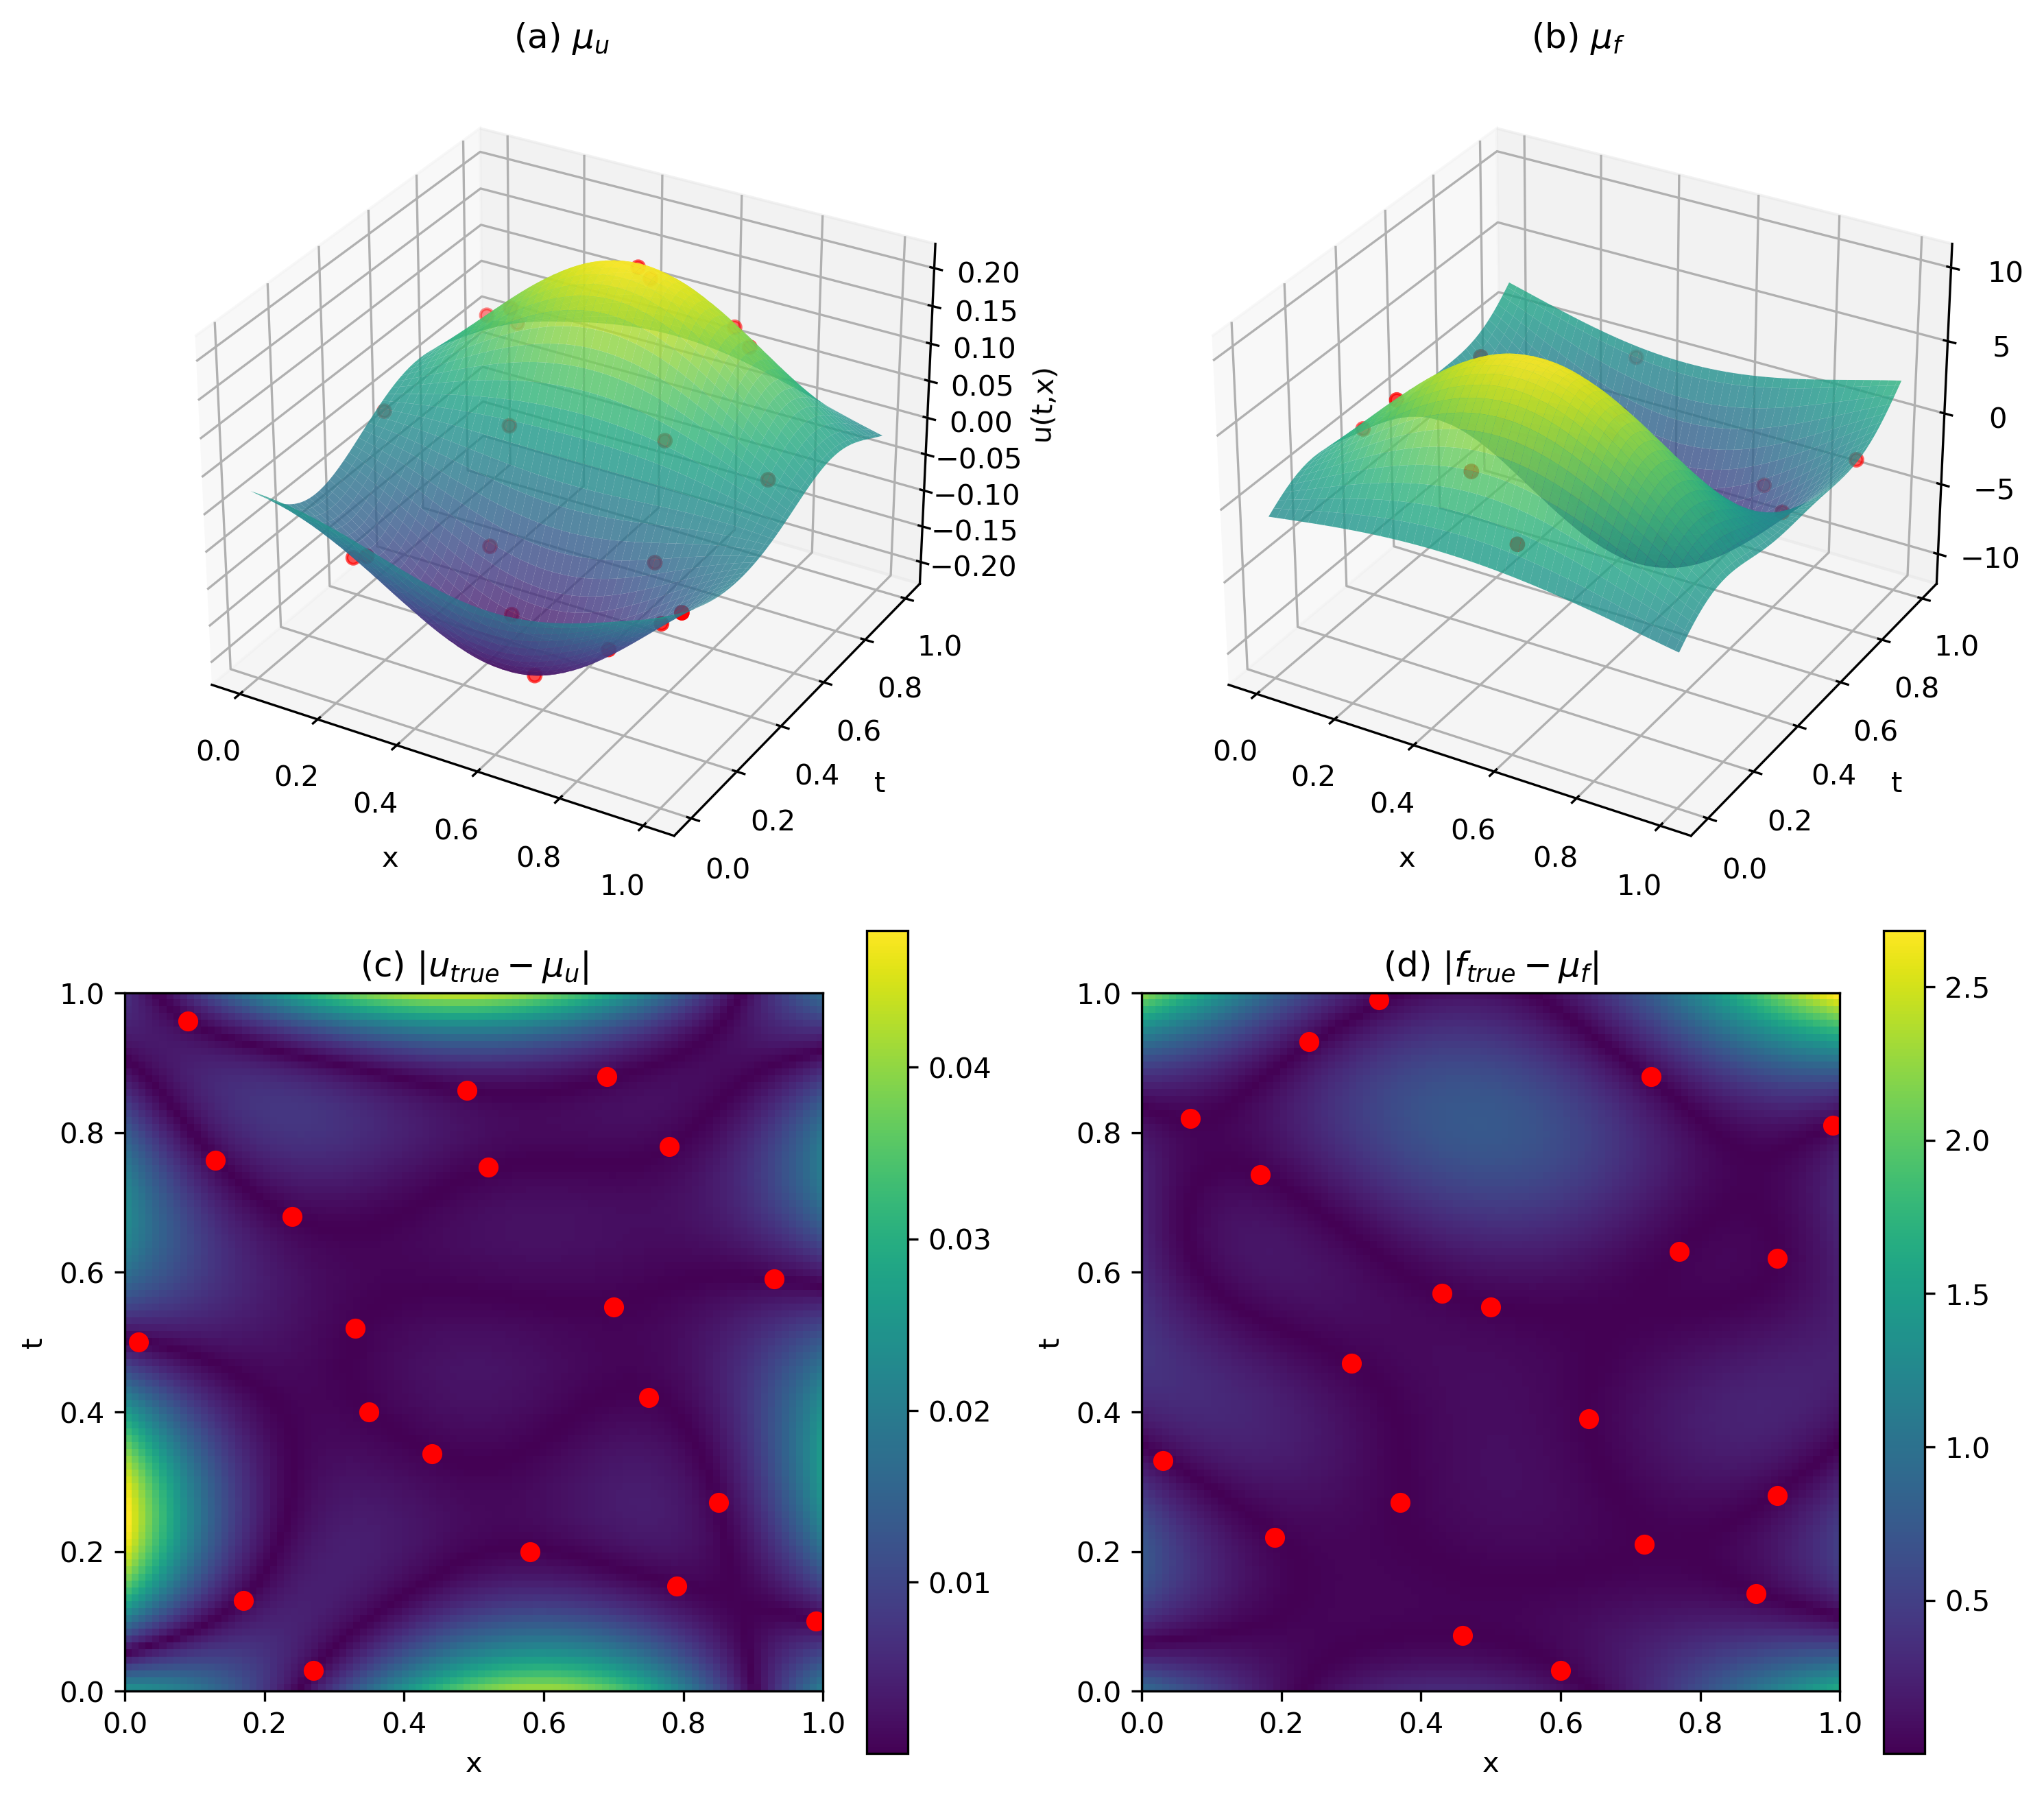
\includegraphics[width=1\textwidth]{../final_examples/poisson/GPy_mean_diff.png}
    \caption{Plots for the vanilla model. (a) \& (b) predictive mean $\bm{\mu_u}$ and $\bm{\mu_f}$} with training points in red. (c) \& (d) difference between the predictive mean $\bm{\mu}$ and the ground truths $u$ and $f$. The MSEs for the vanilla model are $MSE_{u,va} = 9.862  \cdot 10^{-5}$ and $MSE_{f,va} = 0.130$. The relative $L^2$ errors are $L^2_u = 0.0989$ and $L²_f = 0.0728$.
    ~\label{fig:poisson_GPY}
\end{figure}
The area that strikes the most when looking at the prediction with the informed model are the boundaries of the domain. In figure \ref{fig:poisson_boundaries} the slices of the predictive mean together with the ground truth are shown. It is remarkable how precise the model manages to predict the boundaries of the domain, without even using more training points on or near the boundary. 
\begin{figure}
    \centering
    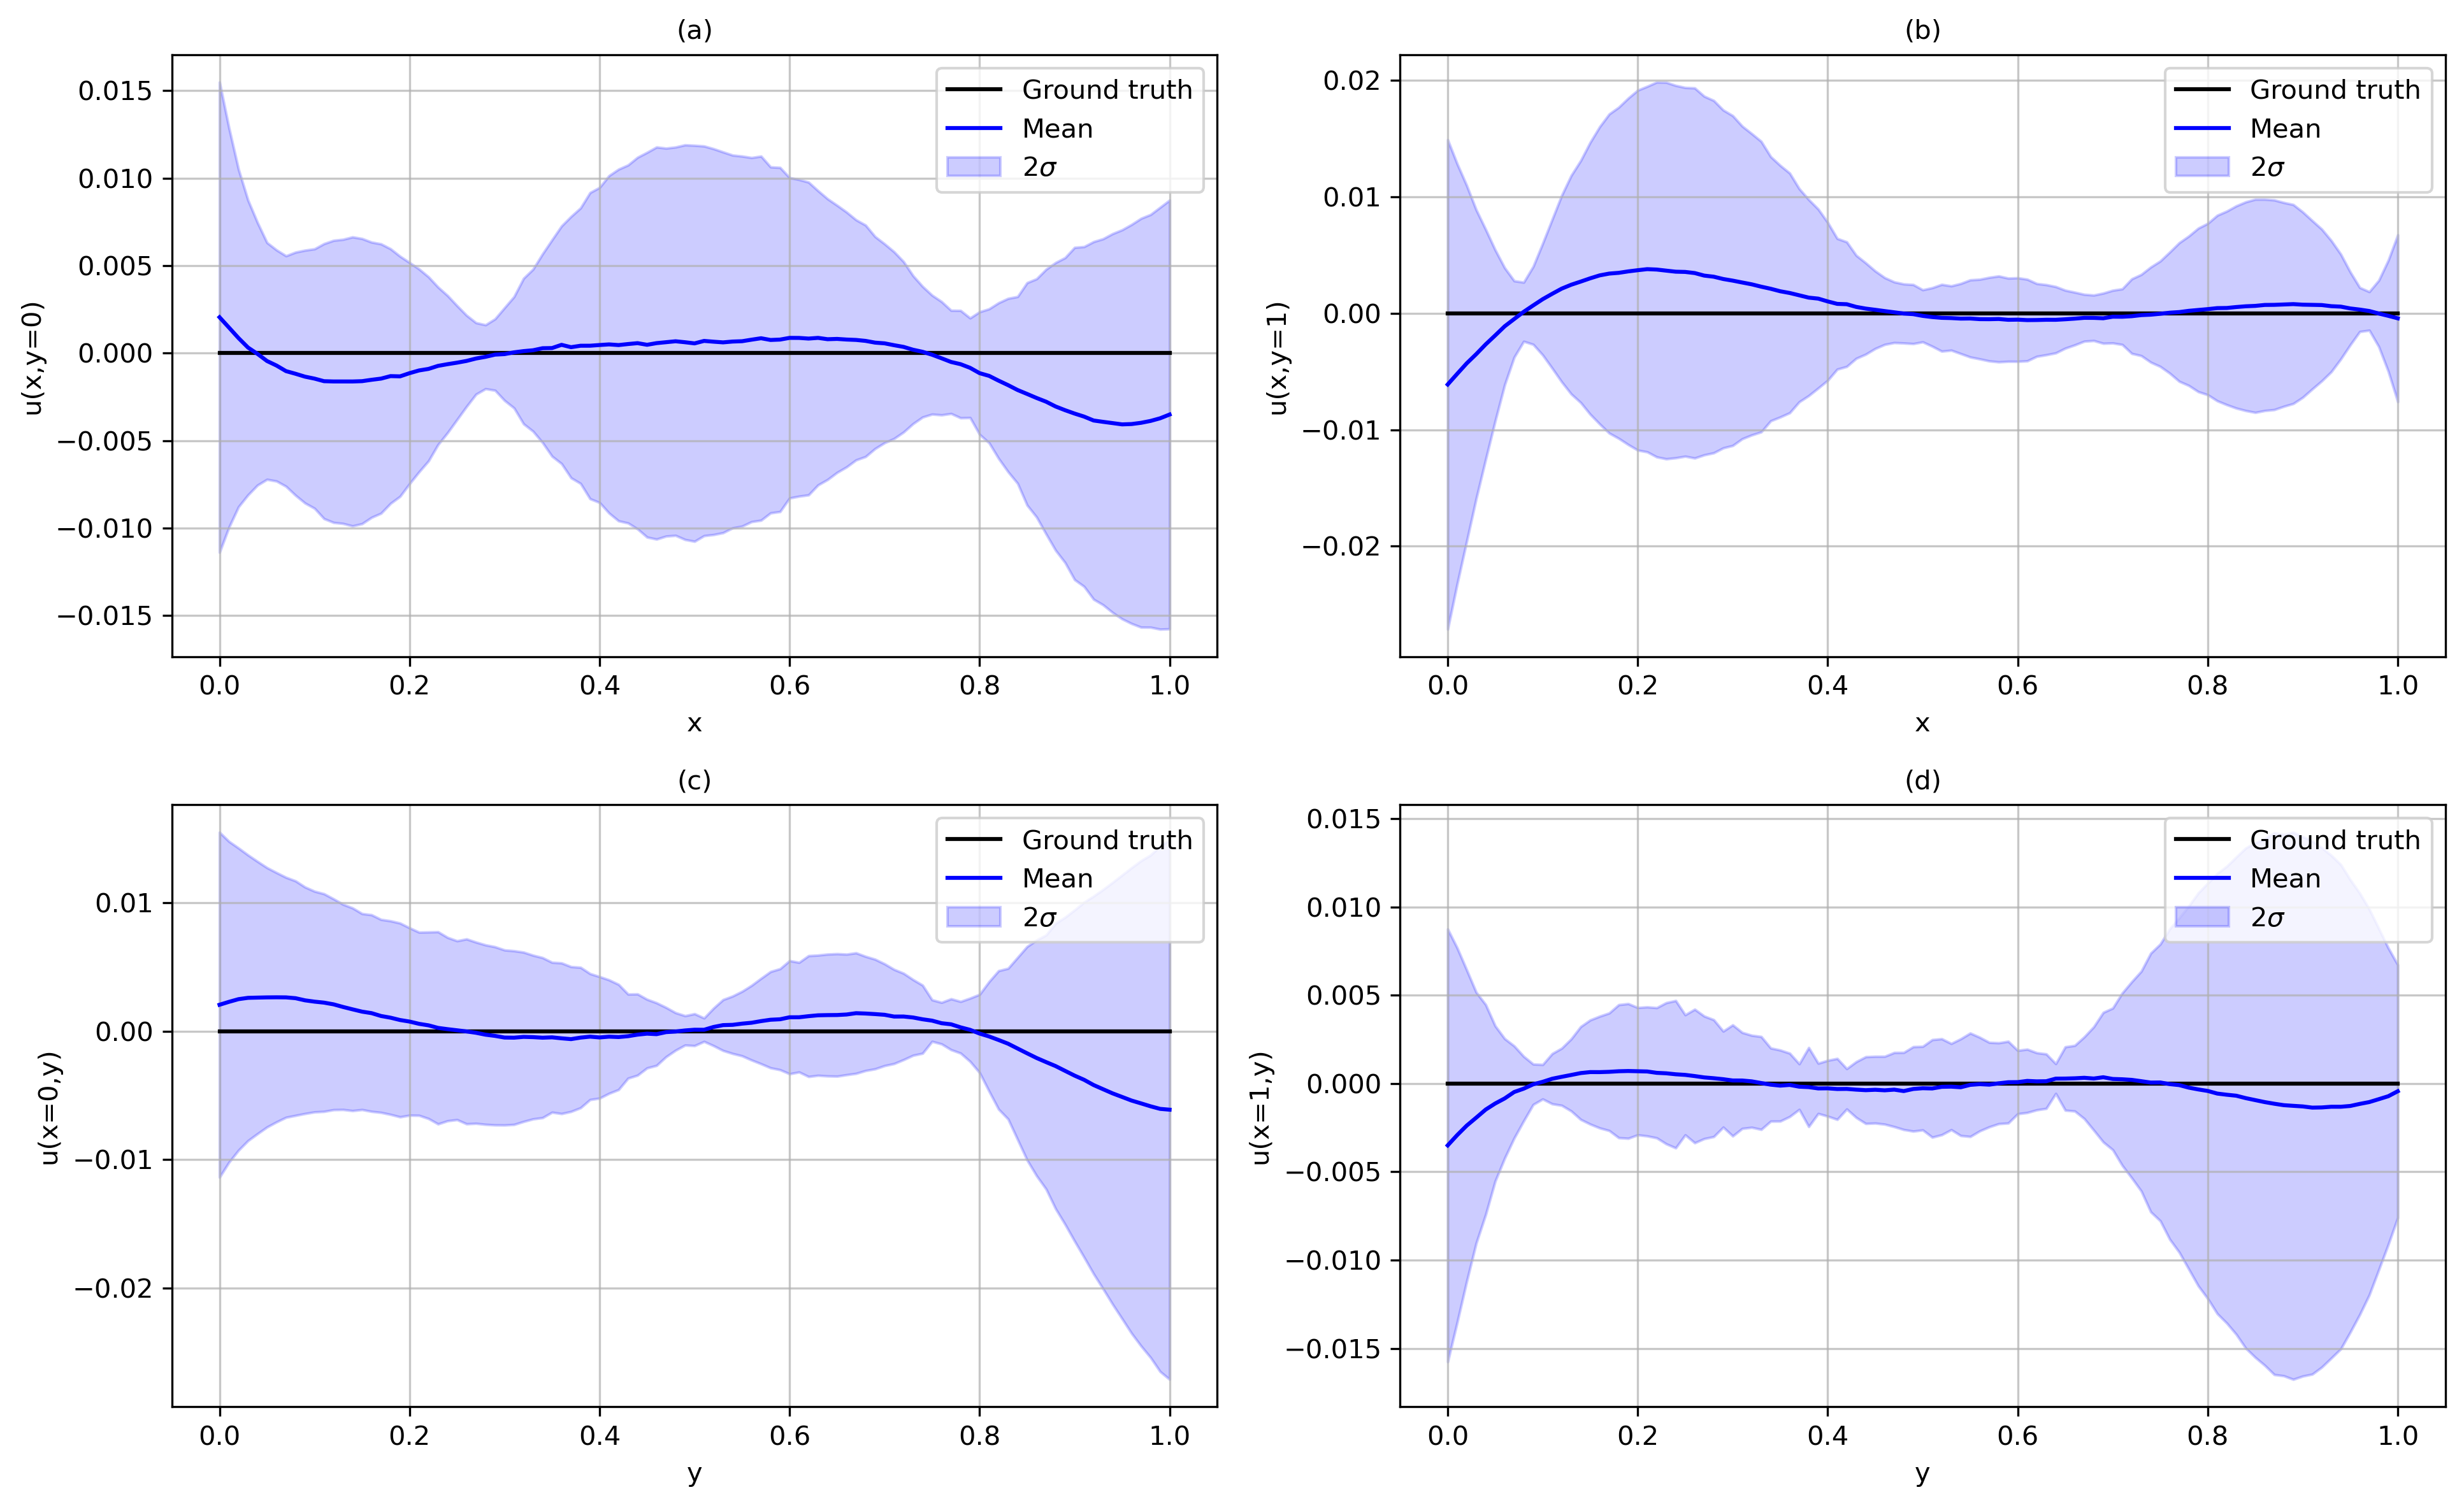
\includegraphics[width=1\textwidth]{../final_examples/poisson/boundaries.png}
    \caption{Plots for the investigation of the domain boundaries}
    \label{fig:poisson_boundaries}
\end{figure}
With this example we can see that the informed models better performance is not only due to the additional hyperparameters. How big the role of the joint GP is, is hard to say, but it is clear that the informed model is notably more accurate than the vanilla model. The most notable difference between the informed and the vanilla model are the predictions at the boundary of the domain. The informed model is able to predict the domain boundaries very accuratly.  \\
\section{Conclusion and Outlook}

\section{Appendix}
\subsection{Numerical implementation of the Kernel}

\bibliographystyle{plain}

\bibliography{library}
\end{document}